\section{Processing Signals}

This section focused on topic already covered in the first part of the lecture. Therefore I left out most of the content and only focused on the new content.


\subsection{Antialiasing Filters}

We already used Gaussian filters for antialiasing. A Gaussian Filter is a infinite response filter. The downside to this type of filter is that it is unstable. We mentioned that a Sinc Filter would be even better (ideal low-pass filter), but it is extremely hard to implement. B-Splines are another type of filter we really like, as they are easy to implement and allow for locally adaptive smoothing.


\subsection{Perspective Projection}

Equally distributed samples in texture space can get unequally distributed when projected into screen space. The optimal filter is spatially variant. \medskip

There are two type of problems that happen when projecting. \textbf{Magnification} happens when the pixel in the texture image maps to an area larger than one pixel. To avoid this we can simply use bilinear interpolation. \textbf{Minification} is the oposite, pixels in the texture image map to areas smaller than one pixel. To deal with this problem we use mipmapping. \medskip

\textbf{Mipmapping} is the process of storing the texture at multiple resolutions (image pyramid) and choosing the resolution level depending on the projected size of the triangle.


\subsection{Geometric Aliasing}

This is another problem that happens at the edges of polygons. Since we our screen space allows for only a limited number of pixels, we end up with a staircase pattern for the edges. To lessen this effect we can apply \textbf{supersampling}. \medskip

Supersampling introduces multiple color samples per pixel, which then are averaged. There are multiple possible sampling patterns, including uniform, jittering, stochastic and poisson. The following shows supersampling using jittering.
\begin{center}
	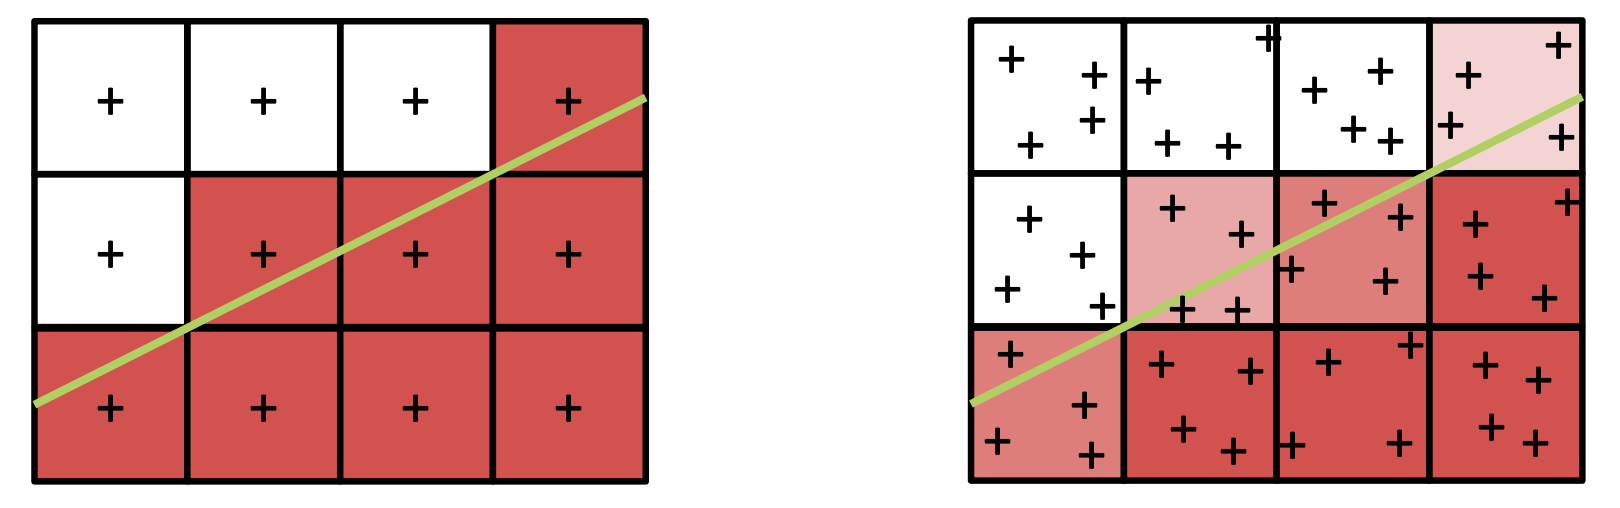
\includegraphics[width=\linewidth]{supersampling.png}
\end{center}
